%@COPYRIGHT VOLLMAIER ALOIS
\definecolor{hellgrau}{RGB}{230, 230, 230}
\lohead{Vollmaier Alois}
\chapter{Informatik}\label{ch:informatik}

\section{Allgemeines}\label{sec:einleitung}
Im folgenden Projektteil werden die Kernbestandteile sowie der nähere Aufbau des informatischen Bereichs dieser Arbeit gezeigt.
Weiters werden wesentliche Elemente der Inbetriebnahme der Maschine dokumentiert und zusammengefasst.
Die Aufteilung dieses XX seitigen Kapitels überstreckt sich über alle signifikanten programmatischen Teile der grafischen Oberfläche, bezeichnet als \textbf{Frontend}, bis hin zu den im Hintergrund arbeitenden Funktionen, welche als \textbf{Backend} zusammengefasst werden.
Auch wird gezeigt, wie einige Teile der \textbf{Hardwarenahen-Programmierung} funktionieren und wie diese mit der Steuerelektronik zusammenarbeiten.
Folglich werden am Schluss der Verlauf der \textbf{Testing-Phase} sowie die Zusammensetzung des \textbf{Teilaufbaus} erläutert.

\section{Zeitplan}\label{sec:zeitplan}
\begin{figure}[hbt!]
    \centering
    \scalebox{0.57}{
    \begin{ganttchart}[
    hgrid style/.style={black, dotted},
    calendar week text={\currentweek},
    vgrid={*6{white, dotted}, *1{black, dashed}},
    x unit=1mm,
    group label font=\bfseries \Large,
    y unit chart=9mm,
    y unit title=12mm,
    time slot format=isodate,
    time slot unit=year
    link/.style={->, thick}
    ]{2019-09-2}{2020-03-15}
        \gantttitlecalendar{year, month=name, week}\\

        \ganttgroup[
        group/.append style={fill=red}
        ]{Backend-Programmierung}{2019-09-02}{2019-11-15}\\ [grid]
        \ganttbar[
        bar/.append style={pattern=north east lines},
        name=KonzeptplanungBack
        ]{Konzeptplanung}{2019-09-02}{2019-09-25}\\ [grid]
        \ganttbar[
        bar/.append style={pattern=north east lines},
        name=Einrichtung - Arbeitsumgebung
        ]{Einrichtung - Arbeitsumgebung}{2019-09-15}{2019-10-1}\\ [grid]
        \ganttbar[
        bar/.append style={pattern=north east lines},
        name=Start-ProgrammierungBack
        ]{Programmierung}{2019-10-05}{2019-11-15}

        \ganttnewline[thick, black]

        \ganttgroup[
        group/.append style={fill=blue}
        ]{Frontend-Programmierung}{2019-11-15}{2020-1-09}\\ [grid]
        \ganttbar[
        bar/.append style={pattern=north east lines},
        name=KonzeptplanungFront
        ]{Konzeptplanung}{2019-11-15}{2019-11-31}\\ [grid]

        \ganttbar[
        bar/.append style={pattern=north east lines},
        name=KonzeptplanungFront
        ]{Anfertigen von Mockup-Skizzen}{2019-11-25}{2019-11-31}\\ [grid]

        \ganttbar[
        bar/.append style={pattern=north east lines},
        name=Start-ProgrammierungFront
        ]{Programmierung}{2019-12-2}{2019-12-22}

        \ganttnewline[thick, black]

        \ganttgroup[
        group/.append style={fill=green}
        ]{Hardwarenahe-Programmierung}{2019-31-31}{2020-2-12}\\ [grid]
        \ganttbar[
        bar/.append style={pattern=north east lines},
        name=KonzeptplanungHard
        ]{Konzeptplanung}{2019-12-31}{2020-1-10}\\ [grid]


        \ganttbar[
        bar/.append style={pattern=north east lines},
        name=Start-ProgrammierungHard
        ]{Programmierung}{2020-1-10}{2020-1-31}

        \ganttnewline[thick, black]

        \ganttgroup[
        group/.append style={fill=green}
        ]{Testen - Aufbauen}{2019-12-22}{2020-02-01}\\ [grid]

        \ganttbar[
        bar/.append style={pattern=north east lines},
        name=Teilaufbau
        ]{Teilaufbau Anfertigung}{2019-12-22}{2020-1-09}\\

        \ganttbar[
        bar/.append style={pattern=north east lines},
        name=Frontend-Testing-Phase
        ]{Frontend-Testing-Phase}{2019-12-31}{2020-1-15}\\

        \ganttbar[
        bar/.append style={pattern=north east lines},
        name=Serial-Testing-Phase
        ]{Serial-Testing-Phase}{2020-1-31}{2020-2-15}

    \end{ganttchart}
    }
    \caption{Zeitplanung - Informatik}
\end{figure}
Das hier gezeigte Bild illustriert, wie der Projektzeitraum aufgeteilt wird.
Um das Zeitfenster des Projekts nicht zu verzögern werden folgende Meilensteine in den Zeitplan implementiert:
\begin{enumerate}
    \item xx.xx.xxxx - Aufgabe XX
    \item xx.xx.xxxx - Aufgabe XX
    \item xx.xx.xxxx - Aufgabe XX
\end{enumerate}
\section{Anforderungen und Ziele}\label{sec:anforderungen-und-ziele}
\subsection{Fronted-Programmierung}\label{subsec:fronted-programmierung}
Im Allgemeinen besteht das Ziel darin, eine benutzerfreundliche grafische Bedienoberfläche zu realisieren, welche schlussendlich im Betrieb der Maschine auf einem 7" Display angezeigt werden soll.
Auf diesem Interface soll es möglich sein, die Steuerung der Maschine zu übernehmen.
Die Möglichkeiten des Benutzers, die Maschine zu bedienen sollen folgende Kernpunkte beinhalten:
\begin{enumerate}
    \item Ausgabe von einzelnen Spielkarten
    \item Konfigurierung von Spielmodi, welche Einstellungen zum Spiel beinhalten
    \item Das Zählen von Punkten und dessen Visualisierung am Display
    \item Ausschalten der Maschine
    \item Übersicht aller vergangenen Spiele
\end{enumerate}
Die wesentliche Anforderung, die Oberfläche einfach und schlicht zu halten, soll im Projekt berücksichtigt werden.
Grundsätzlich steht die sogenannte \textbf{User-Experience}, welche alle Aspekte der Eindrücke eines Nutzers bei der Interaktion mit einem Produkt beschreibt, sowie die \textbf{Funktionalität} bei der Programmierung im Vordergrund.
Um dies zu gewährleisten, sollte eine Voruntersuchung vollzogen werden.

\subsection{Backend-Programmierung}\label{subsec:backend-programmierung}
Wie in der Einleitung bereits erwähnt besteht das Backend aus Tätigkeiten, welche im Hintergrund abgearbeitet werden.
Diese Aufgaben umfassen die Kommunikation des Raspberry PI mit der Ansteuerplatine sowie dem Simulator.

Auch soll im Hintergrund eine sogenannte LOG-Datei, welche wichtige Aktionen protokolliert, automatisch vom Programm generiert werden.
Diese Datei kann z.B. \ beim Debugging-Vorgang notwendig sein bzw. \ dem Entwickler dabei unterstützen, was eine enorme Zeitersparnis mit sich bringt.

Um etwaige Einstellungen der Seriellen Schnittstelle sowie die Definition der Pfade für verschiedene Dateien außerhalb des Programmes vorzunehmen, ist es auch nötig, eine Konfigurationsdatei zu erstellen, welche nach jedem Start vom Programm eingelesen wird.
Mit dieser sogenannten Config-Datei wird auch die Möglichkeit geschaffen, weitere Informationen der Anwendung auch nach einem Neustart der Maschine zu speichern.

Diese hiermit geschaffene Datenpersistenz kommt dem Programm auch bei der zukünftigen Speicherung der Spielmodi oder etwaigen Statistik-Dateien zugute.
Bei einer Realisierung einer Statistik-Datei sollte der Name des ausgewählten Spielmodis, dessen Hintergrundinformationen, Spielernamen und Punkteanzahl Kernbestandteil sein.

Ein weiteres Ziel ist die Internationalisierung der gesamten Software.
Soll eine Software in verschiedenen Ländern eingesetzt werden, ist eine Internationalisierung ein wichtiger Bestandteil der User Experience.
In unserem Fall ist es lediglich notwendig, alle angezeigten Texte zu übersetzen, da keine weiteren Informationen vorhanden sind.

\subsection{Hardwarenahe-Programmierung}\label{subsec:hardwarenahe-programmierung}
Ein weiterer Punkt des Projekts ist die Hardwarenahe-Programmierung.
Aufgrund der Tatsache, das die verwendete Ansteuerplatine über einen ATmega 324PA verfügt, ist es notwendig, eine Programmierung dieses Mikrocontrollers durchzuführen.
Als Basis dafür dienen ankommenden Befehle über der seriellen Schnittstelle.
Ziel ist es also, diese serielle Kommunikation auf dem Mikrocontroller auszuprogrammieren.

\section{Projektspezifische Voruntersuchung}\label{sec:projektspezifische-voruntersuchung}
Damit dem Programmierprozess nichts mehr im Wege steht, ist es notwendig, einige Voruntersuchungen durchzuführen.
Folgend werden einige grundlegende Fragen geklärt und näher erläutert.
\subsection{Auswahl der Arbeitsumgebung}\label{subsec:auswahl-der-arbeitsumgebung}
Das Bearbeiten von Code spielt bei der Programmierung eine elementare Rolle.
Dadurch muss, bevor mit dem Programmierprozess gestartet wird, eine passende IDE ausgewählt werden, welche alle vom Benutzer gestellten Anforderungen erfüllt.
In unserem Fall sind diese im Speziellen:
\begin{enumerate}
    \item Möglichkeiten der Programmierung sowie dem Debuggen eines Remote-Rechners
    \item Nötigsten Features beinhalten
    \item Grafisch Ansprechend
\end{enumerate}
Einer der wichtigsten Punkte dieser Aufzählung ist dabei jedoch die Möglichkeit, Remote-Geräte zu debuggen.
Debugging selbst hilft dem Entwickler bei der Fehlersuche.
Mithilfe der Möglichkeit, das Programm schrittweise auszuführen, ist es auch möglich, die aktelle Wertebelegung von Variablen zu überprüfen.
Dadurch erspart dies enorme Zeit bei der Programmierung.
In unserem Fall ist das Endgerät jedoch nicht der PC, sondern ein Raspberry PI, welcher mit dem Netzwerk über Ethernet verbunden ist.
Es erfordert aber nun die Möglichkeit, das Gerät über das Netzwerk zu debuggen.
\subsubsection{Apache-Netbeans}
Die Netbeans-IDE, bereitgestellt von der Firma Apache, ist eine Open-Source Entwicklungsumgebung, welche selbst in der Programmiersprache Java geschrieben wurde und damit plattformunabhängig ist.
Primär wurde sie entwickelt, um Programme in der Programmiersprache Java zu erstellen.\\
Große Vorteile bringt diese IDE im Bereich der Remote-Programmierung mit sich.
Die Möglichkeit, eine Remote-Plattform einzurichten wurde einfach gelöst und das Arbeiten verläuft meist ohne Probleme.
Auch das einfache Einbinden von Plugins und Bibliotheken zählt zu den Hauptvorteilen von Netbeans.
\subsubsection{Intellij IDEA}
Eine kostenpflichtige Alternative zu Netbeans ist Intellij.
Aufgrund der komplizierten Einrichtung eines Remote-Systems, sowie dessen Handhabung im täglichen Arbeitsprozess wurde deutlich, dass Netbeans im wichtigsten Kriterium besser abschneidet.
Jedoch bring Intellij auch einige Vorteile mit sich.
\begin{enumerate}
    \item Flüssigere Bedienung
    \item Wirkt durchdachter
    \item Zentralere Verwaltung von Plugins
\end{enumerate}
\subsubsection{Fazit}
Natürlich ist es meist Ansichtssache, für welche IDE man sich entscheidet doch in Anbetracht der Vorteile von Netbeans gegenüber Intellij im Bereich der Remote-Programmierung, wurde auch diese IDE für den zukünftigen Arbeitsprozess gewählt.
\subsection{Auswahl des GUI-Frameworks}\label{subsec:auswahl-des-gui-frameworks}
Die Auswahl des für die Anwendung am besten geeigneten GUI-Frameworks, spielt eine wesentliche Rolle in der programmierung von grafischen Anwendungen.
Diese Frameworks stellen meist alle Elemente zur Erstellung einer GUI bereit.
Diese sind z.B.\ Knöpfe, Listen und Textfelder mit denen der Benutzer interagieren kann.
\subsubsection{Swing}
Das bereits in der Standard-Java-Bibliothek verfügbare Java Swing bietet die Möglichkeit komplexe Oberflächen zu erstellen.
Der Aufwand zur Einrichtung hält sich in Grenzen denn im Vergleich zu Java-FX muss hier nicht extern in einem eigenen Programm gearbeitet werden, um die GUI zu erstellen.
Aufgrund der Verfügbarkeit von Java Swing in der Java Bibliothek bieten alle IDE's die Möglichkeit zur erstellung von Oberflächen.
Das etwas veraltete und lieblose Look and Feel von Java Swing brachte uns zur Entscheidung, den Nachfolger, nämlich Java FX, zu verwenden.
\subsubsection{JavaFX}\label{sssec: JavaFX}
JavaFX ist ein GUI-Framework, welches oft als Java-Swing nachfolger betitelt wird.
Hierbei werden im Vergleich zu Java Swing nicht alle GUI Elemente in einer Datei beschrieben, was die Übersichtlichkeit beeinträchtigt, sondern die Beschreibung geschieht in externen FXML-Dateien.
Die Basis dieser FXML-Dateien ist XML, eine Sprache zur Darstellung von Daten in einem von Menschen lesbaren Format.
Näher wird dieses Format im \textit{\autoref{subsec:datenformate-in-java-fx}} erklärt.
Der logische Code hinter der GUI befindet sich jedoch nicht in diesen Dateien, sondern in eigenen Controller-Klassen, welche mit der GUI verknüpft sind.
Dies bringt enorme Vorteile mit sich, denn die strikte Trennung zwischen beschreibenden Elementen der GUI
und dem dahinter stehenden Code ist dadurch möglich.
Benennen darf sich dieses Designkonzept Model-View-Controller. \autoref{subsec:entwurfsmuster-mvc}\\
Auch bieter Java FX die Möglichkeit, separate Stylesheets, also Dokumente, in welchen das Aussehen von Elementen beschrieben wird, zu erstellen.
Diese verbessern das sogenannte Look and Feel drastisch.

\begin{figure}[H]
    \centering
    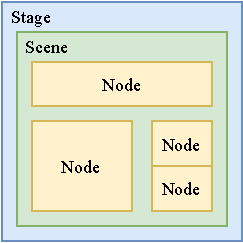
\includegraphics[width=0.3\textwidth]{fig/ainf/JavaFXStageSceneNode.pdf}
    \caption{JavaFX Stage-Scene-Node Übersicht}
    \label{fig:Tool SceneBuilder}
\end{figure}
\subsubsection{Fazit}

\subsection{Projektorganisation}\label{subsec:projektorganisation}
\subsubsection{Projektstruktur in Netbeans}
Eine einheitliche Formatierung und Namensgebung ein Kernbestandteil einer gelungenen Projektplanung.
Dies führt zu einer leichteren Orientierung in fremden aber auch in eigenen Projekten.
Um die Übersichtlichkeit eines Projektes zu verbessern wird nach einer klar definierten Projektstruktur gearbeitet.
Anhand der folgenden Grafik kann die Projektstruktur dieses Projektes abgelesen werden:
\begin{figure}[H]
    \begin{center}
        \begin{forest}
            for tree={
            font=\ttfamily,
            grow'=0,
            child anchor=west,
            parent anchor=south,
            anchor=west,
            calign=first,
            edge path={
            \noexpand\path [draw, \forestoption{edge}]
            (!u.south west) +(7.5pt,0) |- node[fill,inner sep=1.25pt] {} (.child anchor)\forestoption{edge label};
            },
            before typesetting nodes={
            if n=1
            {insert before={[,phantom]}}
            {}
            },
            fit=band,
            before computing xy={l=15pt},
            }
            [<project-root>
            [src
            [data
            ]
            [exception
            ]
            [gui
            ]
            [logging
            ]
            [main
            ]
            [serial
            ]
            [util
            ]
            ]
            [lib]
            [config]
            ]
        \end{forest}
    \end{center}
    \caption{Projektstruktur}
\end{figure}
Der Kopf dieser Struktur beschreibt den Ordner mit dem Namen des Projekts.
Dieser wird auch \lstinline{root-directory} genannt, und ist selbst kein Package.
Auch die Trennung von Sourcecode und externen Dateien spielt eine wesentliche Rolle.
Dadurch erfolgt darunter die Aufteilung in die Ordner \lstinline{src}, \lstinline{lib}, \lstinline{config}.
\\\\
\textbf{Sourcecode}
\\
Im Ordner \lstinline{src} befindet sich der gesamte Sourcecode, wobei in diesem auch wieder eine Aufteilung in Packages erfolgt.
Diese benennen sich in unserem Fall \lstinline{data}, \lstinline{exception}, \lstinline{gui}, \lstinline{logging}, \lstinline{main}, \lstinline{serial}, und \lstinline{util}.
\\\\
\textbf{Bibliotheken}
\\
Oft werden externe Bibliotheken verwendet, welche im Ordner \lstinline{lib} gesammelt werden.
Dabei erleichtert diese Verzeichnishirachie die übersichtlichkeit aller verwendeten Bibliotheken und dessen Versionen.
\\\\
\textbf{Konfigurationsdateien}
\\
In unserem Fall ist es auch notwendig, einen Ordner explizit für Konfigurationsdateien vorzusehen.
Dort können Textresourcen für Sprachvarianten und Konfigurationsdateien für etwaige Aufgaben abgelegt werden.

\subsubsection{Projektstruktur für Maven und Gradle}
Das zuvor genannte Layout der Projekthrachie eignet sich gut für viele Projekte.
Jedoch zeigen sich nach und nach einige Schwachstellen an diesem System.

Einerseits ist das aufwendige Erstellen dieser Hirachie ein Punkt, welcher nicht unerwähnt bleiben soll.
Auch besteht ein Risiko zur Inkonstistenz bei der Namensgebung von Packages oder Bibliotheken. \\
Im Vergleich dazu, schreibt Maven und Gradle eine klar definierte Projektstruktur vor.

\begin{figure}[H]
    \begin{center}
        \begin{forest}
            for tree={
            font=\ttfamily,
            grow'=0,
            child anchor=west,
            parent anchor=south,
            anchor=west,
            calign=first,
            edge path={
            \noexpand\path [draw, \forestoption{edge}]
            (!u.south west) +(7.5pt,0) |- node[fill,inner sep=1.25pt] {} (.child anchor)\forestoption{edge label};
            },
            before typesetting nodes={
            if n=1
            {insert before={[,phantom]}}
            {}
            },
            fit=band,
            before computing xy={l=15pt},
            }
            [<project-root>
            [src
            [main
            [java
            [resources]
            ]
            ]
            [test
            [java
            [resources]
            ]
            ]
            ]
            ]
        \end{forest}
    \end{center}
    \caption{Projektstruktur}
\end{figure}
Trotz alledem wurde auf die althergebrachte Version der Projekterstellung gesetzt.
Grund dafür ist widerum die fehlende Möglichkeit, Remote-Debugging durchzuführen.
Natürlich wäre eine Umstellung in einem finalen Release denkbar.

\section{Grundlagen}\label{sec:grundlagen}
\subsection{Entwurfsmuster Singelton}\label{subsec:entwurdsmuster-singelton}
\subsubsection{Beschreibung}
Das Erzeugungsmuster namens Singelton dient dazu, die Einzigartigkeit eines Objekts sicherzustellen.
Das bedeutet eine Instanz des Objektes ist nur genau einmal im Speicher vorhanden.
Auch bietet eine Klasse, welche nach dem Singelton-Pattern erzeugt wurde, einen globalen Zugriffspunkt über das gesamte Programm.
\subsubsection{Struktur}
Realisiert wird dies durch einen privaten Kontruktor, denn wo keine Zugriffsberechtigung von außen herrscht, kann auch kein Objekt erstellt werden.
Dies bedeutet es liegt eine Kapselung des Konstruktionsprozesses innerhalb der Klasse vor.
Die einzige Möglichkeit, eine Instanz zu erstellen, liefert die statische Methode \lstinline{createInstance()}.
Wurde einmal eine Instanz erzeugt, also der private Konstruktor durch \lstinline{createInstance()} aufgerufen, wird diese erzeugte Instanz in einem statischen Attribut gespeichert.\\
\begin{figure}[H]
    \centering
    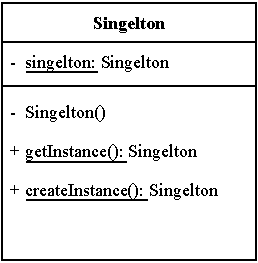
\includegraphics[width=0.25\textwidth]{fig/ainf/Singelton.pdf}
    \caption{UML-Diagramm Singelton}
\end{figure}
Natürlich wird auch ein Zugriffspunkt auf dieses Attribut benötigt.
Implementiert wird dies durch eine weitere statische Methode namens \lstinline{getInstance()}.
Diese Methode ist der einzige Zugriffspunkt auf die Instanz.
\subsubsection{Beispiel}
Das folgende \textit{\autoref{Singelton Code}}, entnommen aus dem \textit{\autoref{subsec:konfiguration}}, zeigt wie Singelton angewendet werden kann.

\lstinputlisting[firstline=22, lastline=38, style=java,caption=Singelton Codebeispiel,label=Singelton Code]{src/data/config/Config.java}

\subsection{Verhaltensmuster Command}\label{subsec:verhaltensmuster-command}
\subsubsection{Beschreibung}
Ziel des Verhaltensmusters Command ist es, den jeweiligen Teilnehmen, welche einen Befehl erzeugt, von dem Teilnehmer der für die Ausführung zuständig ist, zu entkoppeln.
Man kann auch sagen, dass der Teilnehmer, welcher den Befehlsaufruf erzeugt, nicht wissen muss, welcher Teilnehmen den Befehl empfängt oder wo bzw. wann dies geschieht.
Auch kann das tatsächliche Ausführen eines Befehls, aus programmatischer Sicht in einem ganz anderen Thread geschehen, was eine elementare Rolle spielt.
Dieses Verhalten führt zu einer Vereinfachung der Ausführung von komplexeren Tätigkeiten des Programms.
\subsubsection{Struktur}
Das Command-Pattern verfügt meist über verschieden starke Ausprägung.
Im Kern herrscht jedoch immer dasselbe Prinzip, welches in \textit{\autoref{fig:UML-Diagramm Command}} dargestellt wird.
Vorallem die \textbf{Kapselung von Befehlswunsch und Ausführung} steht an erster Stelle.
\begin{figure}[H]
    \centering
    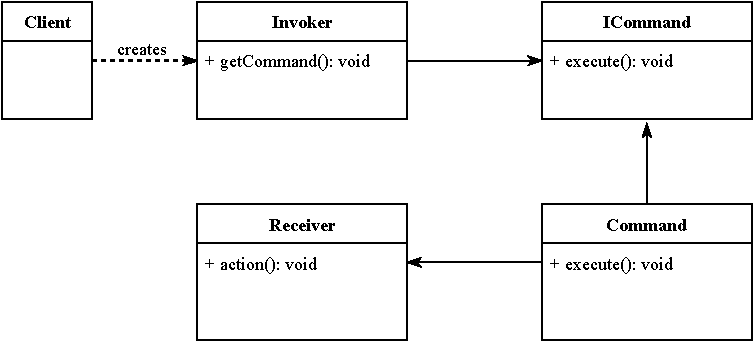
\includegraphics[width=1\textwidth]{fig/ainf/Command.pdf}
    \caption{UML-Diagramm Command}
    \label{fig:UML-Diagramm Command}
\end{figure}
\subsubsection{Beispiel}
\subsection{Entwurfsmuster MVC}\label{subsec:entwurfsmuster-mvc}
\subsubsection{Beschreibung}
Das MVC-Design Pattern, auch Model-View-Controller Design-Pattern, ist eines der weit verbreitetsten Entwurfsmuster.
Es dient zur Strukturierung von Anwendungen und teilt diese in 3 große Bereiche ab, welche strikt voneinander getrennt sind.
Mithilfe dieser Strukturierung fällt es dem Programmierer wesentlich leichter, spätere Änderungen bzw. Erweiterungen am Projekt durchzuführen, da das System nun klar definiert und strukturiert ist.
Auch ist es nun einfacher, parallel an dem Programm zu Arbeiten, denn Ersteller von View und Ersteller des Controllers, also der Berechnungen dahinter, sind nun nicht mehr voneinander abhängig.\\
Jedoch muss bedacht werden, dass Änderungen am Model, direkt an die View weitergegeben werden müssen.
\subsubsection{Struktur}

\begin{enumerate}
    \item \textbf{View}  \\
    Datenrepräsentation\\
    Organisiert alle Kontrollelemente
    \item \textbf{Controller} \\
    Stellt die Verbindung zwischen View und Model her\\
    Verwaltet Benutzerinteraktion und enthält Steuerlogik
    \item \textbf{Model} \\
    Datenrepräsentation\\
    Komplett Abgeschirmt
\end{enumerate}
\begin{figure}[H]
    \centering
    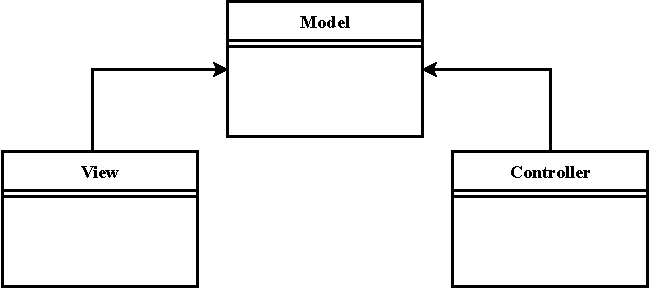
\includegraphics[width=0.8\textwidth]{fig/ainf/ModelViewController.pdf}
    \caption{UML-Diagramm MVC}
    \label{fig:UML-Diagramm MVC}
\end{figure}
\subsection{SceneBuilder}\label{subsec:scenebuilder}
\subsubsection{Beschreibung}
Scenebuilder ist ein umfangreiches GUI-Design-Tool der Firma Gluon.
Verwendet wird es bei Erstellung komplexerer Layouts, denn je komplizierter dieses wird, desto eher stößt man ohne Design-Tool an seine Grenzen.\\\\
Die Verwendung von Tools wie dieses hat mehrere Vorteile.
Einerseits Verbessert sich die Übersichtlichkeit des GUI-Projekts deutlich, da es ab diesem Zeit Zeitpunk möglich ist, den Code hinter der Oberfläche grafisch darzustellen.
Andererseits kann nun, nur mit wenigen Klicks eine für den Endbenutzer ansprechende GUI gebaut werden.\\
Im speziellen hat SceneBuilder weitere wichtige Vorteile wie die direkte Verbindung mit JavaFX und dessen \lstinline{*.fxml} Dateien.
Weiters ist es möglich CSS-Dateien sowie Internationalisierungsdateien einzubinden und diese direkt in SceneBuilder zu verfeinern.
Im wesentlichen ist SceneBuilder, gezeigt in der \autoref{fig:Tool SceneBuilder}, ein performantes Tool und eigent sich optimal für große Projekte wie dieses.
\begin{figure}[H]
    \centering
    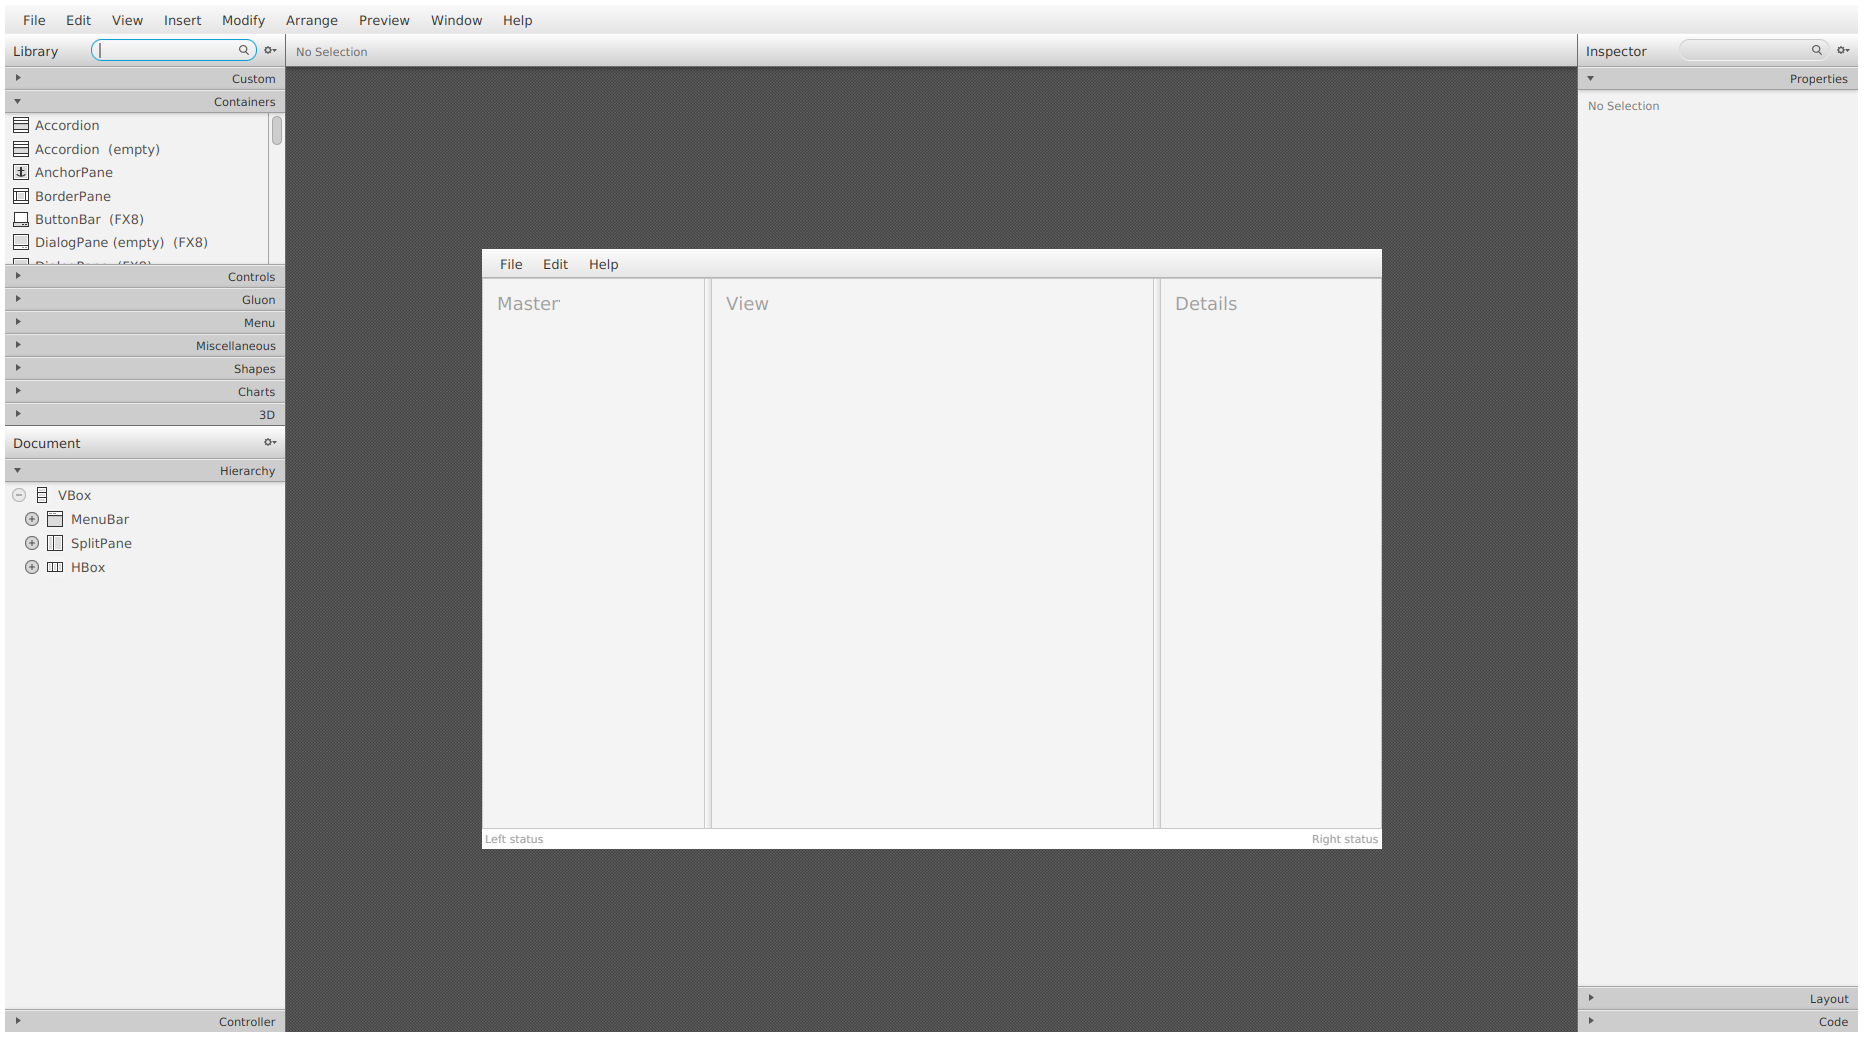
\includegraphics[width=0.8\textwidth]{fig/ainf/SceneBuilder.png}
    \caption{Tool SceneBuilder}
    \label{fig:Tool SceneBuilder}
\end{figure}
\subsubsection{Bibliothek JFoenix}
Sobald nun SceneBuilder als wichtiges Element der Erstellung ausgewählt wurde, kann jetzt ein näherer Blick auf die User-Experience geworfen werden.
Diese sogenannte User-Experience beschreibt, wie der Endbenutzer das Produkt bzw. in unserem Fall die grafische Oberfläche empfindet.
Wird auf diesen Kernpunkt kein Wert gelegt, wird auch niemand erfreut bei der Bedienung sein.\\\\
SceneBuilder bietet bereits einige Grundelemente für Layouts an, doch diese sind nicht ansprechend.
Sie können zwar mir CSS, was im \autoref{sssec: CSS} beschrieben wird, gestaltet werden, dies ist jedoch für alle Elemte schwierig umzusetzten.
Abhilfe schafft dabei die Material-Design Bibliothek von JFoenix.
Diese Bibliothek ist Open-Source und implementiert, wie schon im Namen genannt, Designelemente nach dem von Google entwickelten Material-Design Vorgaben.
Das bedeutet das ohne viel Aufwand, eine höchst ästhetische Oberfläche gebaut werden kann.
Zusätzlich kann man auch hier, eigene CSS-Deklarationen vornehmen, jedoch ist vieles schon vorab definiert\\
Anhand der folgenden \autoref{fig:Rendered Button} soll gezeigt werden, wie nun Elemente, gebaut mithilfe der JFoenix Bibliothek, aussehen.
Angewendet werden die Attribute \lstinline{-fx-border-radius: 20pt;}  \lstinline{-fx-background-radius: 20pt;} und \lstinline{-fx-background-color:grey}
\begin{figure}[H]
    \centering
    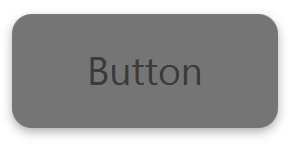
\includegraphics[width=0.4\textwidth]{fig/ainf/RenderedButton.PNG}
    \caption{Gerenderter Button}
    \label{fig:Rendered Button}
\end{figure}
\subsection{Datenformate in Java-FX}\label{subsec:datenformate-in-java-fx}
Im folgenden Kapitel soll auf die Datenpersistenz eingegangen werden.
Speziell in diesem Projekt werden die Datenformate \textbf{XML/FXML}, \textbf{CSS} und \textbf{JSON} verwendet.
Ziel ist es, grundlegende Dinge zu klären und einen kurzen Überblich zu erschaffen.
\subsubsection{XML}
XML(Extensible Markup Language) ist, wie im \autoref{sssec: JavaFX} schon erwähnt, eine Sprache zur Darstellung von Daten in einem von Menschen lesbaren Format.
Damit ist sie also keine Programmiersprache.
Diese XML-Dateien sind zu vergleichen mit normalen Textdokumenten, welche mit einen gewöhnlichen Texteditor geöffnet werden können.

Strukturiert und bezeichnet werden in XML-Dateien die Daten mithilfe von sogenennaten XML-Tags.
Diese Tags stehen in spitzen Klammern und beinhalten den Namen des Datenelements.
Auch ist es notwendig, ein Tag mihilfe eines sogenannten End-Tags zu schließen.
Zwischen diesen Start- bzw. \ End-Tags befindet sich ein Datensatz.
Ein Indikator für ein End-Tag ist ein \lstinline{/}.\\
Zwischen diesen Start- bzw. \ End-Tags befindet sich e
in Datensatz.
Ein Indikator für ein End-Tag ist ein \lstinline{/}.
Anhand der folgenden \autoref{xmlExample} soll gezeigt werden, wie XML-Dateien im inneren aussehen.
% @formatter:off
\begin{lstlisting}[style=XML,caption=XML-Codebeispiel,label=xmlExample]
<?xml version="1.0" encoding="UTF-8"?>
    <email>
        <to>Person1</to>
        <from>Person2</from>
        <heading>Test-Header</heading>
        <body>This is a body :)</body>
    </email>
\end{lstlisting}
% @formatter:on
\subsubsection{FXML}
FXML ist ein auf XML basierendes Datenformat, welches hauptsächlich bei der Erstellung von JavaFX Anwendungen angewendet wird.
Da die Trennung von GUI- und Programmcode bei Java FX nach dem MVC-Pattern \autoref{subsec:entwurfsmuster-mvc}vollzogen wurde, kann erst mithilfe des von Oracle entwickelte Formats ein Layout in einer eigenen Datei gebaut werden.\\\\
Die Struktur und Syntax von FXML Dateien ähnelt der von XML-Dateien.
So werden auch Start- und End-Tags verwendet.
Ein wesentlicher Unterschied ist jedoch bei der Groß-/Kleinschreibung ersichtlich.
Beginnen in FXML-Dateien Elemente mit einem Großbuchstaben, werden diese als Objektdeklarationen behandelt.
Infolgedessen erkennt der FXML-Loader, welcher diese \lstinline{*.fxml} ins Programm lädt, diese Objektdeklarationen nimmt eine dementsprechende Objektbildungen vor.
Sobald diese jedoch mit einem Kleibuchstaben beginnen, definieren sie Eigenschaften.
Eine weitere Besonderheit liegt bei dem Einbinden von Importanweisungen vor.
Dies können mithilfe des Tags \lstinline{<?import ... ?>} ausgeführt werden.\\
\begin{lstlisting}[style=XML,caption=FXML-Codebeispiel,label=fxmlExample]
<?xml version="1.0" encoding="UTF-8"?>
<?import javafx.scene.layout.VBox?>
<?import javafx.scene.control.Label?>

<VBox>
    <children>
    <Label text="Hello ReShuffled :)"/>
    </children>
</VBox>
\end{lstlisting}

\subsubsection{CSS}\label{sssec:CSS}
CSS ist eine Gestaltungs- und Formatierungssprache mit welcher Gestaltungsanweisungen erstellt werden können.
Es soll also beachtet werden, dass CSS nichts mit dem eigentlichen Inhalt der Website oder dem Programm zu tun hat, sondern rein für Design und Stilaspekte verwendet wird.\\
\footfullcite{JavaFX CSS Reference Guide} Für unsere Anwendung bieten JavaFX Cascading Style Sheets (CSS) eine Möglichkeit, die Designziele aus dem \autoref{subsec:fronted-programmierung} umzusetzten und zu verfeinern.
Diese genannte Designsprache stellt eine Erweiterung vom standartisierten CSS mit einigen zusätzlichen Features dar.\\
Grundlegend besteht das Ziel von Java-FX CSS darin, Webprogrammierer, welche CSS bereits für Webanwendungen verwendet haben, die Möglicket zu geben, speziell für JavaFX zugeschnittene Themes zu bauen.
Diese Themes können auf die jeweiligen Kontrollelemente angewendet werden.\\
Eine Besonderheit von JavaFX CSS besteht im Vergleich zur normalen CSS-Sprache.
Alle Elemente, welche mit JavaFX in Verbindung stehen besitzen das Prefix \lstinline{-fx-...}.
Dies lässt sofort auf die Beschreibung eines JavaFX Elements schließen.
\subsection{Datenformat JSON}\label{subsec:json}

\subsubsection{Beschreibung}
Der Name JSON(JavaScript Object Notation) beschreibt neben XML eines der wichtigsten Datenformate zur Sicherstellung der Datenpersistent in der Softwaregeschichte.
Dieser Nachfolger von CSV und INI setzte sich vorallem in der heutigen Datentechnik durch.
Grundlegend ist JSON wiederum ein textuelles Datenformat, welches kompakt und einfach lesbar ist.
Ein weiterer Grund zur Verwendung ist ebenso eine effektive Umwandlung von Daten, also Objekten, Arrays und sonstigen Variablen,  in das JSON-Dateiformat.\\
All diese Merkale sind esentiell wichtig und eröffnen ein breites Spektrum an Verwendungsmöglichkeiten.\\\\
Die Syntax von JSON ist klar definiert und wird ebenfals durch ein Beispiel näher visualisiert.
\begin{lstlisting}[style=json, caption=JSON-Codebeispiel,label=jsonExample]
{
    "employee": {
    "name": "tester",
    "salary": 5432,
    "children": false
    }
}
\end{lstlisting}
\subsubsection{Bibliothek Gson}
Die von Google entwickelte Bibliothek Gson spielt in diesem Projekt eine wichtige Rolle.
Aufgrund enormer Datenmengen ist es zeitaufwändig, JSON Dateien in Java zu erstellen.\\
Eine Hilfe bietet dabei Gson.
Diese unterstützende Bibliothek hilft dem Emtwickler bei der Konvertierung zwischen Java-und JSON-Objekten.
Erstellt wird eine Gson Instanz durch Aufruf des Default-Konstruktors: \lstinline[style=java]{Gson gson = new Gson()}.
Sobald dies vonstatten gegangen ist kann nun entweder mit der Methode \lstinline{toJson} oder mit \lstinline{fromJson} gearbeitet werden.
Diese beiden Methoden stellen die Haupteinstiegspunkte von Gson dar und werden im folgenden Teil erklärt.
\\\\
\textbf{\lstinline{toJson}}
\\
Mithilfe der Mehode \lstinline[style=java]{gson.toJson()} kann direkt aus einem Objekt ein JSON-String erzeugt werden.
Dieser genannte String kann danach je nach belieben in eine Datei geschreiben oder versendet werden.
\\\\
\textbf{\lstinline{fromJson}}
\\
Auch kann der gesamte Prozess mithilfe des Methodenaufrufs \lstinline[style=java]{gson.fromJson()} umgekehr werden.
Hierbei wird aus einem JSON-String ein Objekt erzeugt.
\\
\section{Backend-Programmierung}\label{sec:backend-programmierung}
\subsection{Kommunikation}
\subsubsection{Konzept}
Um erfolgreich Daten zwischen dem Raspberry PI 3B+ und der Platine, welche die Ansteuerung sämtlicher Komponenten übernimmt, zu übertragen, wird ein Kommunikationsprotokoll benötigt.
Dieses Protokoll stellt im engsten Sinne eine Vereinbarung dar, wie die Datenübertragung zwischen zwei oder mehreren Parteien abläuft.
Anforderungen an dieses Protokoll sollen sein:
\begin{enumerate}
    \item einfache Integration in die Zielsysteme
    \item erweiterbarkeit des Protokolls mit geringem Arbeitsaufwand
    \item hohe Sicherheit gegenüber Übertragungsfehler
    \item schnelle Fehlererkennung sowie Fehlerbehebung
\end{enumerate}
Neben standartisierten Protokollen wie Modbus, Feldbus oder CAN-Bus gibt es die Möglichkeit selbst ein sogenanntes propretäres Übertragungsprotokoll zu kreieren.
Dies ist in unserem Fall nötig, um alle Anforderungen abzudecken.
Basierend auf dem Master - Slave Prinzip, wobei der Rasperry PI den Master und die Ansteuerplatine den Slave darstellt, soll ein abgewandeltes Modbus ASCII Protokoll umgesetzt werden.

Zusätzlich soll, um die Anforderung des einfachen Fehlerhandlings zu erfüllen, ein Simulator ausprogrammiert werden, welcher beim Start auf Softwarebebene, den Platz des Slaves bzw. der Ansteuerplatine einnimmt.
Der Startvorgang des Simulators soll mit einer einfachen Modifizierung der Konfigurationsdatei vonstatten gehen.
Die folgende Grafik soll die schematisch die Geräteauswahl darstellen.
\begin{figure}[H]
    \centering
    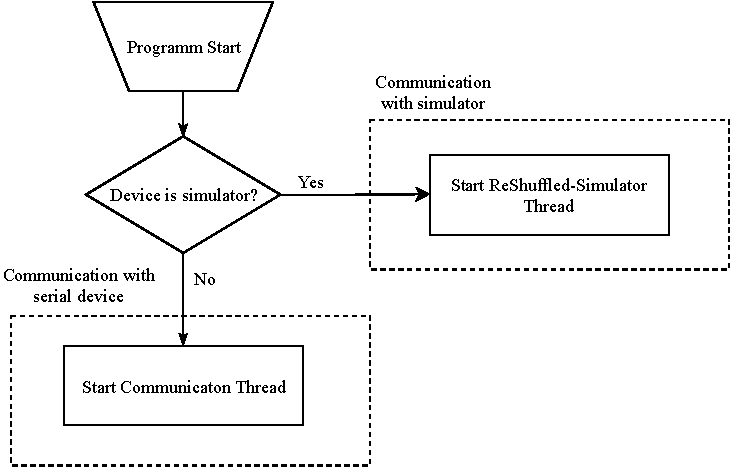
\includegraphics[width=0.8\textwidth]{fig/ainf/DeviceSelection}
    \caption{Schematische Darstellung der Geräteauswahl}
\end{figure}
\subsubsection{Übertragungsprotokoll} \label{sssec:uebertragungsprotokoll}
\begin{table}[H]
    \centering
\resizebox{\textwidth}{!}{%
    \begin{tabular}{|
    >{\columncolor[HTML]{FFFFFF}}l |
    >{\columncolor[HTML]{FFFFFF}}l |
    >{\columncolor[HTML]{FFFFFF}}l |
    >{\columncolor[HTML]{FFFFFF}}l |
    >{\columncolor[HTML]{FFFFFF}}l |}
        \hline
        \textbf{Doppelpunkt :} & \textbf{Daten (ASCII)} & \textbf{Trennzeichen \#} & \textbf{CRC32-Prüfsumme} & \textbf{Semicolon \textbackslash{}n} \\ \hline
        8-Bit & 16-Bit & 8-Bit & 32-Bit & 8-Bit                                \\ \hline
    \end{tabular}
}
    \caption{Visualisierung des Datenakets}
\end{table}
Das verbindugslose Protokoll basiert, wie in der Konzeptbeschreibung bereits erwähnt, auf dem Master-Slave Prinzip.
Außerdem erfolgt die Datenübertragung rein textuell wobei nur Großbuchstaben verwendet werden dürfen.\\\\
Wie aus der oben dargestellten Tabelle zu entnehmen, ist der Aufbau eines Frames klar definiert.
Der eindeutige Start des Datenpakets, welcher mit einem Doppelpunkt (:) eingeleitet wird, sowie das ebenfalls eindeutige Ende, umgesetzt mit einem Line Feed Character (), bringt eindeutige Vorteile mit sich.
Im Gegensatz zu anderen Protokollen wie z.B. Modbus RTU, muss hier nicht auf das Ende des Pakets "gewartet" werden.
Dies führ oft zu Einbußen im Bereich der Performance und ist für uns nicht zielführend.\\\\
Gefolgt von dem Startzeichen folgen nun die Daten.
Diese beinhalten eindeutig definierte Zecichenfolgen, welche verwendet werden um verschiedenste Zustände der Ansteuerplatine auszuführen.
Diese Um auch hier zu wissen, wo sich das der Nutzdaten befindet, schließt das Trennzeichen () diese ab.\\\\
Um nun die Integrität, also die Korrektheit der Daten bei einer Übertragung zu überprüfen, wird im nächsten Schritt eine Prüfsumme verwendet.
Ziel dieser ist es, anhand der Nutzdaten einen Wert zu bilden, welcher danach vom Sender im Frame gespeichert bzw übertragen wird.
Der Empfänger berechnet nun mit dem selben Verfahren die Prüfsumme aus den empfangenen Daten und vergleicht diese mit der Übertragenen Prüfsumme des Senders.
Sind beide Prüfsummen identisch, war die Übertragung erfolgreich und die Daten sind mit großer Wahrscheinlichkeit korrekt.
Stimmen diese nicht überein liegt ein Fehler vor.
Die wichtigsten Arten von Übertragungsfehlern sind:
\begin{enumerate}
    \item Einzelbitfehler (1 Bit verändert)
    \item Burstfehler (ganze Folge von Bits verändert)
\end{enumerate}
Neben einfachen Verfahren wie z.B. dem Paritätsbit-Verfahren gibt es auch Komplexere.
Die zyklische Redundanzprüfung, auch CRC genannt, ist eines davon.
Sie ist realtiv einfach zu realisieren und dennoch wirkungsvoll.
Wichtig beim CRC-Verfahren ist, dass beide Teilnehmen, also Sender und Empfänger, das selbe Generator-Polynom verwenden.
Der Grad des Generatorpolyoms beträgt in unserem Fall 32 (CRC-32).
\subsubsection{Request- und Responsebeispiele}
Folgend wird anhand von tabelarisch aufgelisteten Beispielen gezeigt, wie ein Request mit dem jeweiligen Response zusammenhängt.
Jeder Request sowie Reponse basiert auf der Protokolldefinition aus dem \autoref{sssec:uebertragungsprotokoll}.
\begin{table}[H]
\centering
\resizebox{\textwidth}{!}{%
\begin{tabular}{|l|l|l|c|}
\hline
\rowcolor[HTML]{FFFFFF}
\textbf{Request} & \textbf{Request-String {[}Rx{]}} & \textbf{Aktion} & \multicolumn{1}{l|}{\cellcolor[HTML]{FFFFFF}\textbf{Response-String {[}Tx{]}}} \\ \hline
Init     & IN                                          & Initialisierungs-Zustand     & \multicolumn{1}{l|}{OK oder E\textless{}Code\textgreater{}} \\ \hline
Shutdown & XX                                          & Herunterfahren der Maschine  & --//--                                                      \\ \hline
Shuffle  & SH                                          & Mischen von Karten           & --//--                                                      \\ \hline
Deal     & D\textless{}Anzahl der Karten\textgreater{} & Kartenausgabe je nach Anzahl & --//--                                                      \\ \hline
AutoDeal & A\textless{}Anzahl der Karten\textgreater{} & Automatische Kartenausgabe   & --//--                                                      \\ \hline
\end{tabular}%
}
\caption{Request- und Responsebeispiele Tabellarisch dargestellt}
\end{table}
Aufgrund eines wohldurchdachten Systems bei der Request-Definition, ist es nun möglich, den Pool an verschiedenen Requests explizit zu minimieren.
Dies bezieht sich auf den Vorgang der automatischen Kartenverteilung an jeden den einzelnen Spieler, was mithilfe des Requests \textbf{Deal} und \textbf{AutoDeal} umgesetzt wird.\\
Neben den Request, welche sich rein auf den Ablauf eines Kartenspiels konzentrieren, verfügt der Pool über Requests, welche allgemein zur Funktionalität der Maschine beitragen.
Der Request \textbf{Shutdown} führt jedeglich zu einem Herunterfahren der Maschine.
Auch wird bevor die Maschine in Betrieb genommen wird, der Request \textbf{Init} gesendet.
Dieser hat den Sinn und Zweck, die Maschine in einen Initialisierungszustand zu versetzten.\\
Die genauere Aufarbeitung und Umsetztung sei im \autoref{ssec:konzeptCardDeal} verzeichnet.
\subsubsection{Umsetztung-Datenaustausch}
Zuallererst soll der Ablauf der Kommunikation zwsichen dem Programm und dem Endgeräts, welches über die serielle Schnitstelle verbunden ist, betrachtet werden.
Im ersten Schritt wird auf die Erstellung jedes einzelnen Request eingegangen.\\
Um die Aufgabe der Einbindung von Requests elegant und objektorientiert umzusetzten, stellt die abstrakte Klasse \lstinline[style=java]{Request} den Kopf jedes einzelnen Requests dar.
Dies bedeutet im engsten Sinne, dass jeder einzelne Request eine Abstammung dieser Klasse ist.
Dargestellt wird dies auch durch das generierte UML-Diagramm in \autoref{umlReq}
\begin{figure}[H]
\centering
\vspace{-5mm}
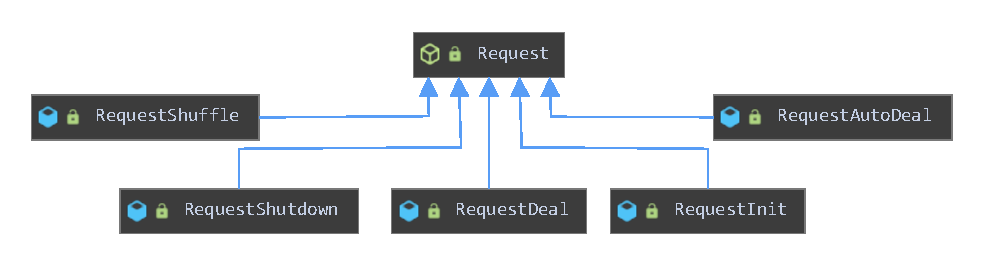
\includegraphics[width=1\textwidth]{fig/ainf/RequestUML.pdf}
\caption{UML-Diagramm-Request-Baum}
\label{umlReq}
\end{figure}
Bevor nun auf jeden einzelnen Request eingegangen wird, soll nun die abstrakte Klasse \lstinline[style=java]{Request} betrachtet werden.
Diese Klasse implementiert die Methoden \lstinline[style=java]{createRequestFrame()}, \lstinline[style=java]{handleRequestSent()} und \lstinline[style=java]{handleResponse()}.\\\\
Wie der Namen der Methoden schon ahnen lässt, ist \lstinline[style=java]{createRequestFrame()} für die Erstellung jedes Request zuständig.
Diese Methode hat hat ist \lstinline[style=java]{protected} somit kann von den abstammenden Requests darauf zugegriffen werden.
\lstinputlisting[firstline=87, lastline=99, style=java,caption=fdsa,label=Gesamte Methode createRequestFrame()]{src/serial/request/Request.java}
Sobald die Methode von einem abstammenden Request aufgerufen wird und der Content, also der Request-String, übergeben wird, überprüft diese Mathode den übergebenen Content.
Sollte dieser leer leet sein wird eine \lstinline[style=java]{IllegalArgumentException} geworfen und die Erstellung des Requests wird somit abgebrochen.
Ist jedoch ein Content vorhanden wird mithilfe der Bibliothek \lstinline{CRC32} eine CRC-32 Prüfsumme erzeugt und in ein hexadezimales Format geparst.
Letztendlich wird danach der Request-String mithilfe eines \lstinline{StringBuilders} zusammengebaut.
Das für die Datenspeicherung im Objekt zuständige Atrribut benennt sich \lstinline[style=java]{private byte[] resFrame} und speichert dessen Daten in ein Byte-Array.\\\\
Weiters verfügt die Klasse die Methode \lstinline[style=java]{handleRequestSent()} welche ausschließlich die Aufgabe hat, den definierten Zeitstempel \lstinline[style=java]{timeMillisFrameSent} zu setzten.
Dieser genannte Zeitstempel ist im nachhinein für das Timeout-Handling von Responses wichtig.\\
Sobald nun ein Response ankommt, kommt die Methode \lstinline[style=java]{handleResponse()} ins Spiel.
Aufgabe dieser ist es, das akommende Response-Objekt, welches im unteren Abschnitt beschreiben wird, in dessen elementaren Daten zu zerlegen.
\lstinputlisting[firstline=36, lastline=42, style=java,caption=fdsa,label=handleResponse() Teilabschnitt]{src/serial/request/Request.java}
Auch soll wiederum in dieser Methode überprüft werden, ob der Content des Frames Fehler aufweist. Dies geschieht wieder mithilfe der in Java implementierten Bibliothek \lstinline{CRC32} und soll nicht näher beleuchtet werden.
Nun wird anhand des zurückkommenden Response-Strings analysiert, wie sich der Request im Zielsystem verhalten hat.
Wie im Protokoll definiert kann nun entweder ein \lstinline[style=java]{OK} oder ein Errorcode mit dem Prefix \lstinline[style=java]{E} zurückkommen.
Der Pool an Codes kann jedoch nur ein Volumen von 9 annehmen, da ansonsten der Frame zu groß wäre.
Umgesetzt wird die Analyse mithilfe einer switch-case-Verzweigung.
\lstinputlisting[firstline=62, lastline=86, style=java,caption=fdsa,label=handleResponse() Teilabschnitt]{src/serial/request/Request.java}
Jeder einzelne Error steht für eine spezielle Fehlerquelle bei der Ausführung.
Eine Übersicht wird in \autoref{ssec:konzeptCardDeal} gegeben.\\\\
Zusätzlich wird in der Klasse \lstinline[style=java]{Request} die \lstinline[style=java]{toString()} Methode überlagert.
Dadurch kann das Request Objekt nun optimal in einen String umgweandelt werden.
\lstinputlisting[firstline=105, lastline=149, style=java,caption=fdsa,label=toString() Methode]{src/serial/request/Request.java}
Nun betrachten wir die spezifischen Request, welche in \autoref{umlReq} zu sehen sind.\\
Im Prinzip ist der Aufbau jeder Request Klasse ähnlich.
Aufgerufen wird der Konstruktor welcher die Methode \lstinline[style=java]{createRequestFrame()} ausführt.
Als Parameter erhält diese Methode den vom Protokoll festgelegten Content.
Als Beispiel soll der Request Shuffle gezeigt werden.
\lstinputlisting[firstline=9, lastline=12, style=java,caption=fdsa,label=toString() Methode]{src/serial/request/RequestShuffle.java}
\textbf{Conclusion:}\\
Somit erhält man nach Erstellung eines Objekts vom gewählten Request-Typ ein vollwärtiges Onjekt mit dem gearbeitet werden kann.
Im folgenden Abschnitt wird nun gezeigt, wie ein Request versendet werden kann.\\\\
Die gesamte Kommunikation wird umgesetzt durch die Klasse \lstinline[style=java]{Communication}.
Diese kann verglichen werden mit einem Wächter, welcher sich um das Senden und Empfangen von Daten kümmert.
Die vom Designpattern Singelton abgeleitete Klasse stellt 2 Threads bereit, wobei einer davon für den Sendung- und einer für den Empfangsvorgang zuständig ist.
Beide werden im privaten Konstruktor der Klasse erstellt und gestartet.
Somit ist ab diesem Zeitpunkt die Verfügbarkeit zur Kommunikation gegeben.\\\\
\textbf{Der CommunicationSendThread:}\\
Nun besteht jedoch das Problem, das  untereinander abgestimmt werden müssen.
Ein wichtiges Beispiel zeigt hierbei das \textbf{Producer-Consumer-Problem} welches in der \autoref{ProducerConsumer} dargestellt wird.
\begin{figure}[H]
\centering
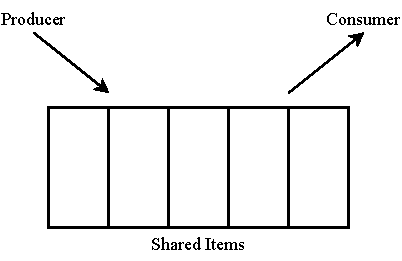
\includegraphics[width=0.45\textwidth]{fig/ainf/ProducerConsumer.pdf}
\caption{Kommunikation Producer-Consumer}
\label{ProducerConsumer}
\end{figure}
Dies bezieht sich auf die gemeinsame Verwendung von Items, da hier Überschneidungen entstehen.
In diesem Fall stellet die sogenannte \lstinline[style=java]{toSentList}, welche als LinkedList vom Typ \lstinline[style=java]{Request} implementiert wurde, die Items dar.
Einerseits müssen hier Requests zur Liste hinzugefügt und andererseits entnommen werden.\\
Um nun die Thread-Sicherheit zu gewährleisten und Deadlocks zu vermeiden, wurde von \lstinline[style=java]{synchronized()} gebrauch gemacht.
Wie schon im oberern Teil beschrieben, bietet die sogenannte \lstinline[style=java]{toSentList} eine gemeinsame Ablage von Requests.
Bei jedem Zugriff wird nun also mit \lstinline[style=java]{synchronized(toSentList)} gearbeitet.
Mithilfe der Methoden \lstinline[style=java]{wait()} und \lstinline[style=java]{notify()} wurde nun eine Möglichkeit geschaffen, um Busy-Waiting, zu vermeiden.
Hier wartet bzw "schläft" der Thread, bis er von außen aktiviert also "aufgeweckt" wird.
Zu sehen ist dies im \autoref{commThreadSync}.
% @formatter:off
\begin{lstlisting}[style=java,caption=Java-Codebeispiel,label=commThreadSync]
try {
    mainLoop:
    while (!Thread.currentThread().isInterrupted()) {
        synchronized (toSentList) {
            LOG.fine("Thread waiting for items ...");
            toSentList.wait();

            if (!toSentList.isEmpty()) {
            ....
            }
        }
    }
}
catch (Exception ex) {
    LOG.warning(ex, Thread.currentThread().getName() + " exception");
}
finally {
    LOG.info(Thread.currentThread().getName() + " ended");
}
\end{lstlisting}
% @formatter:on
Hinzugefügt kann ein Item über die Methode \lstinline[style=java]{public void sendRequestExecutor (Request req)} werden.
Diese Methode, welche nach dem Command-Verhalensmuster (\autoref{subsec:verhaltensmuster-command}) gestaltet wurde, fügt ledeglich ein Element zur Liste hinzu und "weckt" den Thread mit \lstinline[style=java]{notifyAll()}.
\lstinputlisting[firstline=67, lastline=72, style=java,caption=fdsa,label=toString() Methode]{src/serial/Communication.java}
Befindet sich nun etwas in der \lstinline[style=java]{toSentList}, beginnt der Thread zu arbeiten.
Ein Loop zur Sendung eines Request kann einfach anhand des \autoref{commThreadSend} erklärt werden.
% @formatter:off
\begin{lstlisting}[style=java,caption=Java-Codebeispiel,label=commThreadSend]
if (!toSentList.isEmpty()) {
    pendingRequest = toSentList.removeFirst();
    LOG.fine("sending request " + pendingRequest.getMreqFrame());
    serial.writeString(pendingRequest.getMreqFrame());
    pendingRequest.handleRequestSent();
}
\end{lstlisting}
% @formatter:on
Vorerst wird der wartende Request in dem Attribut \lstinline[style=java]{Request pendingRequest} gespeichert und von der Liste gelöscht.
Danach kann dieser über die serielle Schnitstelle versendet werden.
Dies erfolgt mithilfe der Hilfsmethode \lstinline[style=java]{serial.writeString()} welche im \autoref{sssec:deviceSelection} beschrieben wurde.\\\\
Nun soll auf den ankommenden Response gewartet werden.
Auch hier wird eine LinkedList implementiert.
Diese besteht jedoch nicht aus Request-Objekten, sondern aus sogenannten Response-Objekten.
In jedem einzelnen Objekt vom Typ \lstinline[style=java]{Response} befindet sich der Frame, gepeichert in dem Attribut \lstinline[style=java]{byte [] resFrame}, und ein Zeitstempel namens \lstinline[style=java]{long timeMillisCreatedAt}.\\\\
Wird nun vom CommunicationReceiveThread, welcher später beschrieben wird, empfangen und zur \lstinline[style=java]{responseList} hinzugefügt, entfernen die folgenden Zeilen Code den Request von der Liste und speichern diesen.
% @formatter:off
\begin{lstlisting}[style=java,caption=Java-Codebeispiel,label=commThreadSend]
res = responseList.removeFirst();
if (!responseList.isEmpty()) {
    LOG.warning("response list should be empty, but " + responseList.size() + " items in list");
    responseList.clear();
}
\end{lstlisting}
% @formatter:on
Mithilfe des Methodenaufrufs \lstinline[style=java]{pendingRequest.handleResponse(res)} wird nun, wie oben beschreiben, der Response weiter verarbeitet.\\\\
Sollte jedoch kein Response ankommen, versucht das Programm, sofern in der Konfigurationsdatei ein zweiter Versuch erlaubt ist, den selben Response nochmals zu senden.
Ist dies nicht der Fall, wird eine \lstinline[style=java]{SerialException} geworfen.
% @formatter:off
\begin{lstlisting}[style=java,caption=Java-Codebeispiel,label=commThreadSend]
if (responseList.isEmpty()) {
    if (Config.getInstance().getConfigSerial().isSecondTryAllowed()) {
        sendRequestExecutor(pendingRequest);//send second response
        continue mainLoop;
    }
throw new SerialException("request timeout, mssing response"); // if second try isnt allowed throw serial exception
}
\end{lstlisting}
% @formatter:on
Somit wäre ein Kommunikationsloop abgeschlossen und der \lstinline[style=java]{communicationSendThread} wartet wieder auf ankommende Requests des Programms.\\\\
\textbf{Der CommunicationReceiveThread:}\\
Nun sollte jedoch das Empfangen eines Response näher beschrieben werden.
Dieser Thread holt sich vorerst den InputStream und liest danach die Zeichen ein.
Sollte ein unerwartetes Zeichen ankommen, wird in dien Log-Datei eine Warunung geschrieben.
Werden die ankommenden Daten nun als vollwärtigen Request empfunden, fügt der Thread diesen zur oben genannten \lstinline[style=java]{responseList} hinzu und weckt den Thread.
\subsubsection{Umsetztung-Geräteauswahl} \label{sssec:deviceSelection}

\subsubsection{Serial-Simulator}
\subsection{Logging}
\subsubsection{Konzept}
Logging ist nach dem Debugging selbst, dass zweitwichtigeste Mittel um einzelne Programmbausteine oder das gsamte Programm auf Fehler zu untersuchen.
Mithilfe einer Log-Datei können z.b aktuelle Wertebelegungen im Detail dargestellt werden.
Natürlich kann dies auch mithilfe einer Konsolenausgabe über \lstinline[style=java]{System.out.println()} realisiert werden, jedoch ist eine Verwendung von Logging-Frameworks immer sinvoller.\\\\
\textbf{Gründe für die Verwendung von Logging-Frameworks}\\
Als Beispiel kann mithilfe einer Log-Datei auch ein Benutzer, welcher nicht über die Möglichkeit verfügt, den Quellcode einzusehen, einzelne Fehler erkennen(vorrausgesetzt diese Möglichkeit ist durch das Programm geschaffen).
Auch ist nun die Persistenz der Logging-Einträge gegeben.
Dies bedeuted, es kann nun sichergestellt werden, dass diese Einträge auf dem System gespeichert werden und nach einem Neustart verfügbar sind.
Nutzt man diese Art von Protokollierung kann man außerdem die Genauigkeit der Erfassung genau parametrisieren.\\
Zusammengefasst bringt das Erstellen einer Log-Datei mithilfe eines Logging-Frameworks ein großes Feld an Möglichkeiten mit sich.\\\\
In unserem Fall
\subsubsection{Integration in das Programm}
\subsection{Konfiguration}\label{subsec:konfiguration}
\subsubsection{Konzept}
\subsubsection{Datenmodelle}
\subsubsection{Verwahrung am Zielsystem}

\subsection{Statistiken}
\subsubsection{Konzept}
\subsubsection{Datenmodelle}
\subsubsection{Verwahrung am Zielsystem}

\subsection{Controllerklassen}
\subsubsection{Grundlagen}
\subsubsection{StartupController}
\subsubsection{MainController}
\subsubsection{HomeController}
\subsubsection{StatsController}
\subsubsection{About- und HelpController}


\section{Frontend-Programmierung}
\subsection{Designkonzept}



\begin{lstlisting}[style=java,caption=Java Codebeispiel,label=Model]
public class Model extends Observable{
private int counter;
public Model() {
}
public int getCounter() {
return countDown;
}
public void increment() {
if (counter > 0) {
counter++;
}
notifyObservers();
}
\end{lstlisting}

\begin{lstlisting}[style=java,caption=Die Klasse View,label=View]
public class View implements Observer {
private Model model;
private Stage stage;
private Label label;
private Button countButton;
public View(Model model, Stage stage) {
this.model = model;
this.stage = stage;
label = new Label("Counter: " + model.getCounter());
btIncrement = new Button("Increment by 1");
stage.setScene(new Scene(new VBox(label, countButton)));
model.addObserver(this);
}
@Override
public void update(Observable o, Object arg) {
label.setText("Counter: " + model.getCounter());
\end{lstlisting}
\subsection{Utility Klassen}
\subsubsection{AlertUtil}
\subsubsection{GuiUtil}
\subsection{Implementierung von CSS}
\subsubsection{StartupCSS}
\subsubsection{HomeCSS}
\subsection{Internationalisierung}
\subsubsection{Gründe der Umsetzung}
\subsubsection{Integration in das Interface}
\subsubsection{Ressourcen Manager}
\subsubsection{Resource Utility}
\subsubsection{Bereitgestellte Ressources Bundles}

\section{Hardwarenahe-Programmierung}
\subsection{Einrichtung des Mikrocontrollers}
\subsection{Konzept und Ablaufdiagramm zur Kartenausgabe} \label{ssec:konzeptCardDeal}
\section{Teilaufbau}
\subsection{Auswahl des Zielsystems}
\subsubsection{Arduino}
\subsubsection{Raspberry PI}
\subsection{Auswahl des Displays}
\subsection{Montage und Testaufbau}
\subsection{Konfiguration des Zielsytsems}
\subsubsection{Betriebssystem}
\subsubsection{Speichermedium}
\subsubsection{Touchpanel}
\subsubsection{SSH und SFTP}
\subsubsection{Autostart realisiert durch Services}

\section{Probleme - Verbesserungsmöglichkeiten - Zusammenfassung}
\subsection{Probleme}
\subsubsection{Probleme bei der Implementierung von JavaFX}
\subsubsection{Kommunikation zwischen Controllern}
\subsection{Verbesserungsmöglichkeiten}
\subsubsection{Online Update-Möglichkeit der Software}
\subsubsection{Smartphone-Interface zum Zählen der Punkte}
\subsection{Zusammenfassung}